\documentclass[conference,column]{IEEEtran}
\usepackage[a4paper,left=2.54 cm,right=2.54 cm,top=2.54 cm,bottom=2.54 cm]{geometry}
\usepackage{graphicx}
\usepackage{epstopdf}
\usepackage{amsmath}
\usepackage{amssymb}
\usepackage{ textcomp }
\epstopdfDeclareGraphicsRule{.pdf}{.png}
\DeclareGraphicsExtensions{.png,.pdf}


\begin{document}
\title{Segment Tree, the Amazing Data Structure}
\author{\IEEEauthorblockN{	Snahashis Roy  \\Roll: 1603091 \\Computer Science \& Engineering\\RUET\\ \and  Sadman Sakib\\Roll: 1603090\\Computer Science \& Engineering\\RUET}}

\maketitle


\begin{abstract}
The topic is about the data structure, segment tree. Segment Tree is a data structure which is used in cases where there are multiple range queries on array and modifications of elements of the same array. For example, finding the sum of all the elements in an array from indices L to R, or finding the minimum value of all the elements in an array from indices L to R. In short, segment tree is used for range query and range update.


Segment Tree is basically a binary tree used for storing the intervals or segments. Each node in the Segment Tree represents an interval. Each node has a parent node (except root node) and has maximum two child nodes. It has a value which represents the specific information in that interval of the node. For example, sum the elements or minimum value in that interval~\cite{typeee}.


Suppose, we are given an array A[]. There are two types of queries. They are:
\begin{enumerate}
	\item Update all elements from A[L] to A[R] by adding 1 with each of them.
	\item Find the sum of all element from A[L] to A[R].
\end{enumerate}


If the above problem is solved in iterative approach the time complexity will be 
O(query x arrayLength). But segment tree can reduced the time complexity into O(query x log(arrayLength)). For larger constraint like query = $10^5$ and arrayLength = $ 10^5 $
segment tree gives us a better result than iterative approach.

\end{abstract}

\section{Introduction}
Segment Tree is basically a binary tree used for storing the intervals or segments. Thus each node of this tree has zero or two children. Nodes having zero child are called leaf nodes and represent the single element from the given array for which Segment tree would be built. Each node of the tree will hold information about a range from the given array. The closer the node to root, the more range it covers. Here left child will hold information for left half of the parent range and right child will hold info for remaining right half~\cite{def}. 


Considering an array A of size N and a corresponding Segment Tree T:
\begin{enumerate}
\item The root of T will represent the whole array A[0:N - 1].
\item Each leaf in the Segment Tree T will represent a single element A[i] such that 0 $\leq$ i \textless N.
\item The internal nodes in the Segment Tree T represents the union of elementary intervals A[i:j] where\\ 0 $\leq$ i \textless j \textless N.
\end{enumerate}		


The root of the Segment Tree represents the whole array A[0:N - 1]. Then it is broken down into two half intervals or segments and the two children of the root in turn represent the A[0:$\frac{(N - 1)}{2}$+1 : (N - 1)] and . So in each step, the segment is divided into half and the two children represent those two halves. So the height of the segment tree will be log2N. There are N leaves representing the N elements of the array. The number of internal nodes is N - 1. So, a total number of nodes are 2 x N - 1. 


A Segment Tree can be built using recursion (bottom-up approach). Start with the leaves and go up to the root and update the corresponding changes in the nodes that are in the path from leaves to root. Leaves represent a single element. In each step, the data of two children nodes are used to form an internal parent node. Each internal node will represent a union of its children’s intervals. Merging may be different for different questions. So, recursion will end up at the root node which will represent the whole array. Once the Segment Tree is built, its structure cannot be changed. We can update the values of nodes but we cannot change its structure~\cite{type}.   

\section{Methodology}

In this paper, our methodology is mainly divided into 3 parts. They are:
\begin{enumerate}
\item To build a segment tree
\item To update value
\item To make query
\end{enumerate}

\subsection{\textbf{To build a segment tree}}


We start with a segment arr[0 . . . n-1]. and every time we divide the current segment into two halves(if it has not yet become a segment of length 1), and then call the same procedure on both halves, and for each such segment, we store the sum in the corresponding node~\cite{typee}. 


\begin{center}
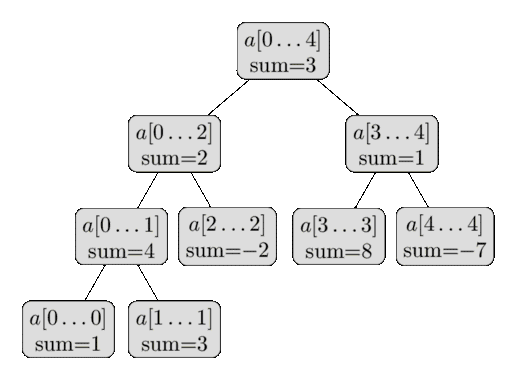
\includegraphics[scale=0.60]{1.png}
\end{center}
\begin{center}
Fig.: Segment Tree
\end{center}



\textbf{C++ implementation of the above idea}
\begin{center}
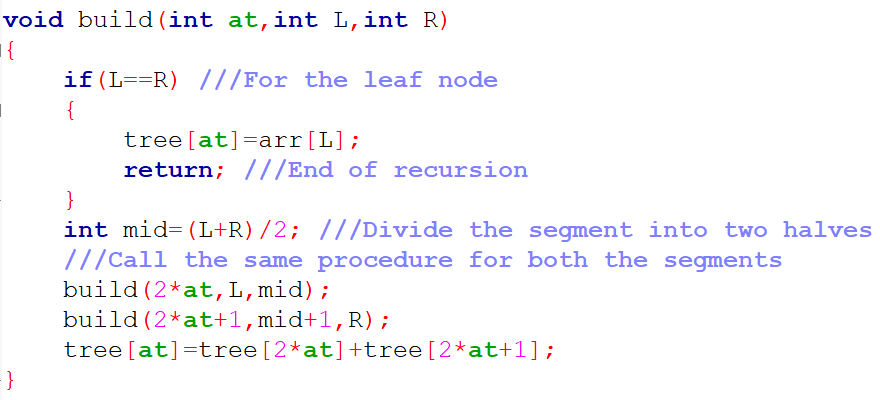
\includegraphics[scale=0.60]{2.png}
\end{center}

Time Complexity: O( n x log(n) ) where, n is the size of array.

\subsection{\textbf{To update value}}



Like tree construction update can be done recursively. We are given index ‘id’ which is to be updated and new value ‘val’. We will start from the root of the tree. Each time we will divide the segment into two halves if our target index is in between the segment and thereby we will go either left or right.
Gradually, we will get our target index and will update it by new value ‘val’.



\textbf{C++ implementation of the above idea}
\begin{center}
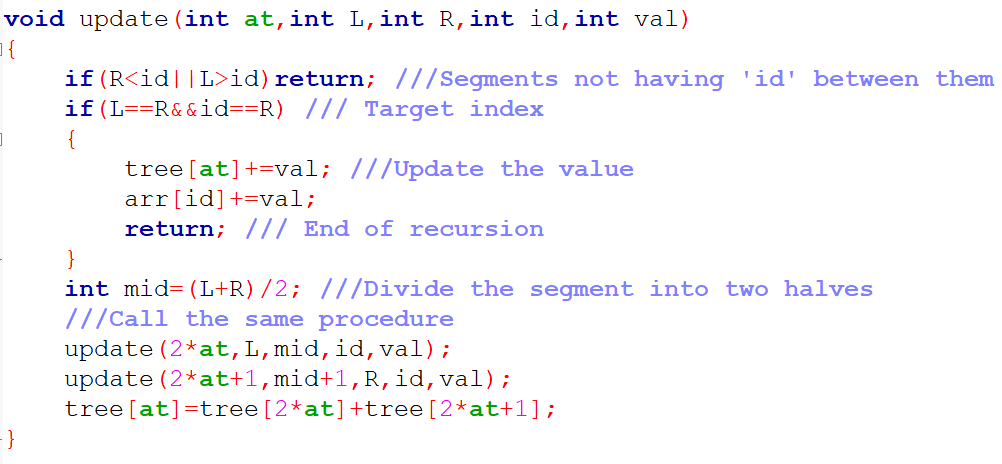
\includegraphics[scale=0.50]{3.png}
\end{center}

Time Complexity: O(log(n)) where, n is the size of array.


\subsection{\textbf{To make query}}


Like tree construction and update, query can be done recursively. We are given ‘L’ and ‘R’. We have to calculate the summation from arr[L] to arr[R]. We will start from the root. Each time we will follow one of the three cases. They are:\\
\textbf{Case-1:} If our current segment is fully included in between L-R we will simply return it’s summation from segment sum. \\
\textbf{Case-2:} If our current segment is fully excluded from L-R we will simply return 0. \\
\textbf{Case-3:} If our current segment is partially included in between L-R we will divide it into two halves and gradually go to each halves



\textbf{C++ implementation of the above idea}
\begin{center}
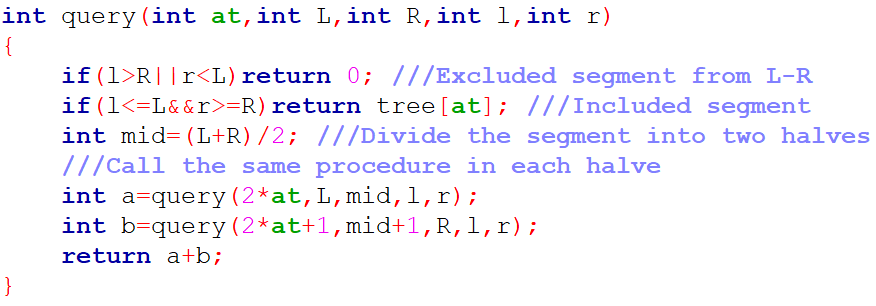
\includegraphics[scale=0.60]{4.png}
\end{center}

Time Complexity: O(log(n)) where, n is the size of array.


\begin{thebibliography}{10}
\bibitem{typeee}
MD. Mahbubul Hasan, “Programming Contest Data Structure and Algorithm”, pp. 133-137, 2016.
\bibitem{def}
https://www.geeksforgeeks.org/segment-tree-set-1-sum-of-given-range/
\bibitem{type}
https://www.hackerearth.com/practice/data-structures/advanced-data-structures/segment-trees/tutorial/
\bibitem{typee}
https://codeforces.com/blog/entry/15890
\end{thebibliography}

\end{document}